\documentclass[12pt]{article}
	
%______________________PREAMBULO_________________________

%----------------------Paquetes--------------------------
\usepackage{amsmath,amssymb,amsfonts,latexsym,cancel} % Paquetes de símbolos adicionales.
\usepackage[spanish,es-tabla]{babel} % Idioma español
\usepackage[utf8]{inputenc} % Paquete que nos permite usar los acentos y otros símbolos, directamente del teclado.
\usepackage[T1]{fontenc} % Cambia el tipo de letra
\usepackage{times} % Tipo de letra Times New Roman
\usepackage{graphicx} % Paquete para el manejo de gráficos y figuras en el documento.
\usepackage{geometry} % Permite el manejo de los margenes
\usepackage{fancyhdr} % Permite colocar y manejar el encabezado
\usepackage[breaklinks,colorlinks=true,linkcolor=black,citecolor=blue, urlcolor=blue]{hyperref} % Crea hipervinculo entre secciones y el indice
\usepackage{pstricks}
%\usepackage{multicol}
%\usepackage{mathpazo} %fuente palatino
%\usepackage{xcolor}
%\usepackage[shortlabels]{enumitem}
%-------------Paquetes para el formato de las citas-------
%\usepackage[hyphens]{url}
%\usepackage{float}
%\usepackage{cite}
%\usepackage{wrapfig}

%-----------------------------ayuda de paquetes--------------------

\spanishdecimal{.}

%------------------------Margenes----------------------------

\newgeometry{bottom = 2.5 cm, top = 2.5 cm, left = 2 cm, right = 2 cm} % Modifica el margen {Abajo, Arriba, Izquierda, Derecha

%----------------------------Interlineado----------------------------------

%\doublespacing
%\onehalfspace
%\singlespace
%\spacing{1.5} % Permite personalisar a gusto
%\setlength{\parskip}{2cm} % Es el espacio entre parrafos

%-----------------------------Sangria---------------------------------------

\setlength{\parindent}{0 cm} % Manipula la sangria

%---------------------Portada------------------

%\title{
%\begin{figure}[h!]
		
%	\centering
%	
\includegraphics[width=\linewidth]{Nom_UAdeC_FCFM.png}  			
			
%\end{figure}
%\huge \textbf{LABORATORIO DE FISICA 3}\\\LARGE TITULO PRACTICA\\}
%\author{ \Large \textbf{Profesor:}\\
%\Large \textbf{Alumno:} Oscar Joel Castro Contreras}
%\date{\today}

%--------------Encabezado y pie de pagina--------------------

\pagestyle{fancy}%Coloca el encabezado en el documento
\lhead[]{Física 3}%Encabezado izquierda
\rhead[]{Oscar Joel Castro Contreras}%Encabesado derecha
%\chead[]{}%Encabesado central
\renewcommand{\headrulewidth}{0.08 pt}%Coloca linea al pie de pagina

%\lfoot[]{PI}%Pie de pagina izquerdo
%\rfoot[]{PD}%Pie de pagina derecho
\cfoot[]{\thepage}%Pie de pagina central
\renewcommand{\footrulewidth}{0.08 pt}%Coloca linea al pie de pagina

%-----------------------------------------------------------------------------

	\begin{document}
		
		\begin{titlepage}
		
			\centering
			{\bfseries
			\begin{figure}[h!]
				\centering
				
\includegraphics[width=\linewidth]{Nom_UAdeC_FCFM.png} 				
			\end{figure}
			\par}
			\vspace{2cm}
			{\scshape\LARGE FÍSICA 3 \par}
			\vspace{3cm}
			{\scshape\Huge \textbf{Tarea 1 - Campo Eléctrico} \par}
			\vfill
			{\LARGE \textbf{Profesora:} Ricardo Pérez Martinez \par}
			\vspace{3cm}
			{\LARGE \textbf{Alumno:} Oscar Joel Castro Contreras \par}
			\vfill
			{\Large \today \par}
			\thispagestyle{empty}
			%\thispagestyle{fancy}
			
		\end{titlepage}
	
		\newpage
		
		\tableofcontents		
		
		\newpage
		
		\section*{Formulas:}\label{sec:Formulas}
			$$ k_e = 8.99 \times 10^9 \frac{Nm^2}{C^2} \quad \epsilon_0 = 8.8542 \times 10^{-12} \frac{C^2}{Nm^2} $$
			$$ \rho = \frac{Q}{V}, \quad \sigma = \frac{Q}{A}, \quad \lambda = \frac{Q}{L} $$
			$$ dq = \rho dV, \quad dq = \sigma dA, \quad dq = \lambda dL $$
			\begin{align}
				k_e &= \frac{1}{4\pi\epsilon_0} \nonumber \\
				\vec{E} &= \frac{\vec{F_e}}{q_0} \\
				\vec{F_e} &= q_0 \vec{E} \\
				\vec{F_e} &= k_e \frac{|q||q_0|}{r^2} \hat{r} \\
				\vec{E} &= k_e \frac{|q|}{r^2} \hat{r} \\
				\vec{E} &= k_e \int \frac{dq}{r^2} \hat{r}
			\end{align}

		\section{Problema 1:}\label{sec:Problema1}
			Tres cargas puntuales están alineadas a lo largo del eje $ x $. La carga $ q_1 = 3\mu C $ está en
			el origen, y la carga $ q_2 = -5\mu C $ se encuentra en $ x = 0.2m $. La carga $ q_3 = -8\mu C $.
			¿Dónde está situada $ q_3 $ si la fuerza neta sobre $ q_1 $ es de $ 7N $ en la dirección negativa
			del eje $ x $?.
			\begin{center}
				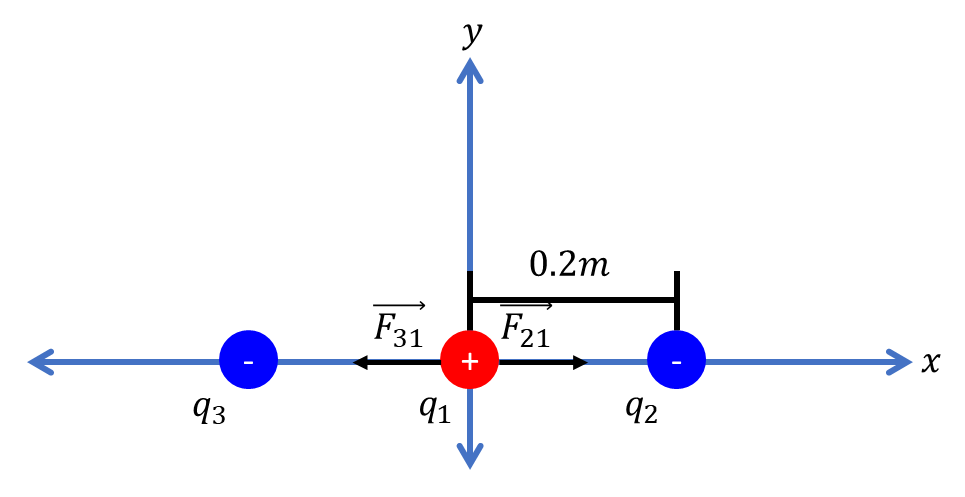
\includegraphics[width=.7\textwidth]{Imp1t1.png}
			\end{center}
			$$ q_1 = 3\mu C = 3 \times 10^{-6}C, \quad q_2 = -5\mu C = -5 \times 10^{-6}C, \quad q_3 = -8\mu C = -8 \times 10^{-6}C $$
			$$ r_{21} = 0.2m, \quad r_{31} = ? $$
			$$ \vec{F_{n1}} = -7N\hat{i} $$ \\
			$$ \vec{F_{n1}} = \vec{F_{21}} + \vec{F_{31}} $$
			$$ \vec{F_{21}} = k_e \frac{q_2q_1}{(r_{21})^2} \hat{r}, \quad \vec{F_{31}} = k_e \frac{q_3q_1}{(r_{31})^2} \hat{r} $$
			$$ \vec{F_{n1}} = k_e \frac{|q_2||q_1|}{(r_{21})^2} \hat{i} - k_e \frac{|q_3||q_1|}{(r_{31})^2} \hat{i} $$ \\
			$$ \vec{F_{21}} = 8.99 \times 10^9 \frac{Nm^2}{C^2} \left( \frac{(5 \times 10^{-6}C)(3 \times 10^{-6}C)}{(0.2m)^2} \right) \hat{i} $$
			$$ \vec{F_{21}} = 8.99 \times 10^9 \frac{Nm^2}{C^2} \left( \frac{1.5 \times 10^{-11}C^2}{0.04m^2} \right) \hat{i} $$
			$$ \vec{F_{21}} = 8.99 \times 10^9 \frac{Nm^2}{C^2} \left( 3.75 \times 10^{-10} \frac{C^2}{m^2} \right) \hat{i} $$
			$$ \vec{F_{21}} = 3.37125N \hat{i} $$ \\
			$$ \vec{F_{31}} = -8.99 \times 10^9 \frac{Nm^2}{C^2} \left( \frac{(8 \times 10^{-6}C)(3 \times 10^{-6}C)}{(r_{31})^2} \right) \hat{i} $$
			$$ \vec{F_{31}} = -8.99 \times 10^9 \frac{Nm^2}{C^2} \left( \frac{2.4 \times 10^{-11}C^2}{(r_{31})^2} \right) \hat{i} $$
			$$ \vec{F_{31}} = -\left( \frac{0.21576Nm^2}{(r_{31})^2} \right) \hat{i} $$ \\
			$$ \vec{F_{n1}} = 3.37125N \hat{i} - \left( \frac{0.21576Nm^2}{(r_{31})^2} \right) \hat{i} $$
			$$ -\left( \frac{0.21576Nm^2}{(r_{31})^2} \right) \hat{i} = \vec{F_{n1}} - 3.37125N \hat{i} $$
			$$ -\left( \frac{0.21576Nm^2}{(r_{31})^2} \right) \hat{i} = -7N \hat{i} - 3.37125N \hat{i} $$
			$$ -0.21576Nm^2 \hat{i} = (-10.37125N \hat{i})(r_{31})^2 $$
			$$ (r_{31})^2 = \frac{-0.21576Nm^2 \hat{i}}{-10.37125N \hat{i}}$$
			$$ r_{31} = \sqrt{2.08 \times 10^{-3}m^2}$$
			$$ r_{31} = 1.4 \times 10^{-1}m, \quad \underline{r_{31} = -1.4 \times 10^{-1}m} $$ \\

		\section{Problema 2:}\label{sec:Problema2}
			Dos cargas puntuales se localizan sobre el eje $ y $ como sigue: la carga $ q_1 = -1.5nC $
			está en $ y = -0.6m $ y la carga $ q_2 = 3.2nC $ se halla en el origen $ (y = 0) $. ¿Cuál es la
			fuerza total (magnitud y dirección) ejercida por estas dos cargas sobre una tercera
			carga $ q_3 = 5nC $ que se ubica en $ y = -0.4m $?.
			\begin{center}
				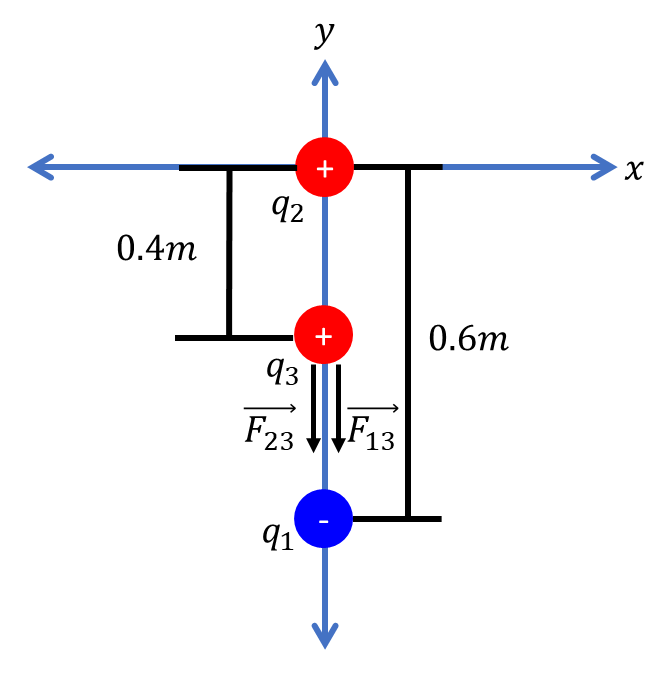
\includegraphics[width=.5\textwidth]{Imp2t1.png}
			\end{center}
			$$ q_1 = -1.5nC = -1.5 \times 10^{-9}C, \quad q_2 = 3.2nC = 3.2 \times 10^{-9}C, \quad q_3 = 5nC = 5 \times 10^{-9}C $$
			$$ r_{23} = 0.4m, \quad r_{13} = 0.6m - r_{23} = 0.2m $$ \\
			$$ \vec{F_{t3}} = \vec{F_{23}} + \vec{F_{13}} $$
			$$ \vec{F_{23}} = k_e \frac{q_2q_3}{(r_{23})^2} \hat{r}, \quad \vec{F_{13}} = k_e \frac{q_1q_3}{(r_{13})^2} \hat{r} $$
			$$ \vec{F_{t3}} = -k_e \frac{|q_2||q_3|}{(r_{23})^2} \hat{j} - k_e \frac{|q_1||q_3|}{(r_{13})^2} \hat{j} $$ \\
			$$ \vec{F_{23}} = -8.99 \times 10^9 \frac{Nm^2}{C^2} \left( \frac{(3.2 \times 10^{-9}C)(5 \times 10^{-9}C)}{(0.4m)^2} \right) \hat{j} $$
			$$ \vec{F_{23}} = -8.99 \times 10^9 \frac{Nm^2}{C^2} \left( \frac{1.6 \times 10^{-17}C^2}{0.16m^2} \right) \hat{j} $$
			$$ \vec{F_{23}} = -\frac{1.4384 \times 10^{-7}Nm^2}{0.16m^2} \hat{j} $$
			$$ \vec{F_{23}} = -8.99 \times 10^{-7}N \hat{j} $$ \\
			$$ \vec{F_{13}} = -8.99 \times 10^9 \frac{Nm^2}{C^2} \left( \frac{(1.5 \times 10^{-9}C)(5 \times 10^{-9}C)}{(0.2m)^2} \right) \hat{j} $$
			$$ \vec{F_{13}} = -8.99 \times 10^9 \frac{Nm^2}{C^2} \left( \frac{7.5 \times 10^{-18}C^2}{0.04m^2} \right) \hat{j} $$
			$$ \vec{F_{13}} = -\frac{6.7425 \times 10^{-8}Nm^2}{0.04m^2} \hat{j} $$
			$$ \vec{F_{13}} = -1.685625 \times 10^{-6}N \hat{j} $$ \\
			$$ \vec{F_{t3}} = \vec{F_{23}} + \vec{F_{13}} $$
			$$ \vec{F_{t3}} = -8.99 \times 10^{-7}N \hat{j} - 1.68562 \times 10^{-6}N \hat{j} $$
			$$ \vec{F_{t3}} = -2.6 \times 10^{-6}N \hat{j} $$
			$$ \underline{F_{t3} = 2.6 \times 10^{-6}N \; a \; 270^0} $$ \\

		\section{Problema 3:}\label{sec:Problema3}
			Dos cargas puntuales iguales y positivas, $ q_1 = q_2 = 2\mu C $ se localizan en $ x = 0, y =
			0.3m $ y $ x = 0, y = -0.3m $ respectivamente. ¿Cuáles son la magnitud y la dirección
			de la fuerza eléctrica total (neta) que ejercen estas cargas sobre una tercera carga,
			también puntual, $ Q = 4\mu C $ en $ x = 0.4m, y = 0 $?.
			\begin{center}
				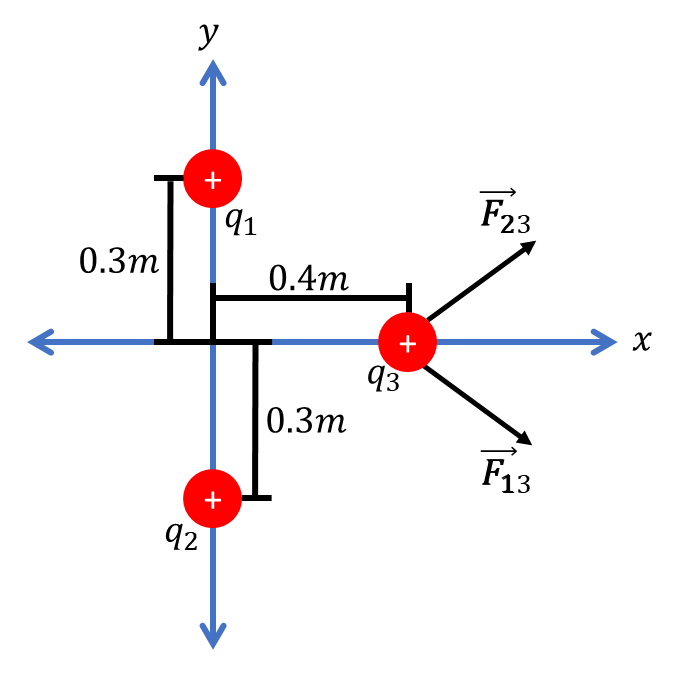
\includegraphics[width=.5\linewidth]{Imp3t1.png} 
			\end{center}
			$$ q_1 = q_2 =  2\mu C = 2 \times 10^{-6}C, \quad q_3 = 4\mu C = 4 \times 10^{-6}C $$
			$$ r_{13} = \sqrt{(0.3m)^2 + (0.4m)^2} = 0.5m $$
			$$ r_{23} = \sqrt{(-0.3m)^2 + (0.4m)^2} = 0.5m $$ \\
			$$ \vec{F_{n3}} = \vec{F_{13}} + \vec{F_{23}} $$
			$$ \vec{F_{13}} = \vec{F_{13}}x + \vec{F_{13}}y, \quad \vec{F_{23}} = \vec{F_{23}}x + \vec{F_{23}}y$$
			$$ \vec{F_{13}} = k_e \frac{|q_1||q_3|}{(r_{13})^2} \hat{i} - k_e \frac{|q_1||q_3|}{(r_{13})^2} \hat{j}, \quad 
			\vec{F_{23}} = k_e \frac{|q_2||q_3|}{(r_{23})^2} \hat{i} + k_e \frac{|q_2||q_3|}{(r_{23})^2} \hat{j}$$
			$$ \vec{F_{n3}} = \left( k_e \frac{|q_1||q_3|}{(r_{13})^2} \hat{i} - k_e \frac{|q_1||q_3|}{(r_{13})^2} \hat{j} \right) 
			+ \left( k_e \frac{|q_2||q_3|}{(r_{23})^2} \hat{i} + k_e \frac{|q_2||q_3|}{(r_{23})^2} \hat{j} \right) $$ \\
			$$ \vec{F_{13}} = 8.99 \times 10^9 \frac{Nm^2}{C^2} \left( \frac{(2 \times 10^{-6}C)(4 \times 10^{-6}C)}{(0.5m)^2} \right) \hat{i}
			- 8.99 \times 10^9 \frac{Nm^2}{C^2} \left( \frac{(2 \times 10^{-6}C)(4 \times 10^{-6}C)}{(0.5m)^2} \right) \hat{j}  $$
			$$ \vec{F_{13}} = 8.99 \times 10^9 \frac{Nm^2}{C^2} \left( \frac{8 \times 10^{-12}C^2}{0.25m^2} \right) \hat{i}
			- 8.99 \times 10^9 \frac{Nm^2}{C^2} \left( \frac{8 \times 10^{-12}C^2}{0.25m^2} \right) \hat{j} $$
			$$ \vec{F_{13}} = \left( \frac{0.07192Nm^2}{0.25m^2} \right) \hat{i} - \left( \frac{0.07192Nm^2}{0.25m^2} \right) \hat{j} $$
			$$ \vec{F_{13}} = 0.28768N \hat{i} - 0.28768N \hat{j} $$ 
			$$ \vec{F_{13}}x = 0.28768N \hat{i}, \quad \vec{F_{13}}y = -0.28768N \hat{j} $$\\
			$$ \vec{F_{23}} = 8.99 \times 10^9 \frac{Nm^2}{C^2} \left( \frac{(2 \times 10^{-6}C)(4 \times 10^{-6}C)}{(0.5m)^2} \right) \hat{i}
			+ 8.99 \times 10^9 \frac{Nm^2}{C^2} \left( \frac{(2 \times 10^{-6}C)(4 \times 10^{-6}C)}{(0.5m)^2} \right) \hat{j}  $$
			$$ \vec{F_{23}} = 8.99 \times 10^9 \frac{Nm^2}{C^2} \left( \frac{8 \times 10^{-12}C^2}{0.25m^2} \right) \hat{i}
			+ 8.99 \times 10^9 \frac{Nm^2}{C^2} \left( \frac{8 \times 10^{-12}C^2}{0.25m^2} \right) \hat{j} $$
			$$ \vec{F_{23}} = \left( \frac{0.07192Nm^2}{0.25m^2} \right) \hat{i} + \left( \frac{0.07192Nm^2}{0.25m^2} \right) \hat{j} $$
			$$ \vec{F_{23}} = 0.28768N \hat{i} + 0.28768N \hat{j} $$
			$$ \vec{F_{13}}x = 0.28768N \hat{i}, \quad \vec{F_{13}}y = 0.28768N \hat{j} $$\\
			$$ \vec{F_{n3}} = (\vec{F_{13}}x + \vec{F_{13}}y) + (\vec{F_{23}}x + \vec{F_{23}}y) $$
			$$ \vec{F_{n3}} = (\vec{F_{13}}x + \vec{F_{23}}x) + (\vec{F_{13}}y + \vec{F_{23}}y) $$
			$$ \vec{F_{n3}} = (0.28768N \hat{i} + 0.28768N \hat{i}) + (-0.28768N \hat{j} + 0.28768N \hat{j}) $$
			$$ \vec{F_{n3}} = 0.57536N \hat{i} + 0 \hat{j} $$
			$$ \underline{F_{n3} = 0.57536N \; a \; 0^0} $$

		\section{Problema 4:}\label{sec:Problema4}
			Dos cargas puntuales están situadas sobre el eje $ x $ del modo siguiente: la carga
			$ q_1 = 4nC $ está en $ x = 0.2m $ y la carga $ q_2 = 5nC $ está en $ x = -0.3m $. ¿Cuáles son
			la magnitud y la dirección de la fuerza total ejercida por estas dos cargas, sobre una
			carga puntual negativa $ q_3 = -6nC $ que se halla en el origen?.
			\begin{center}
				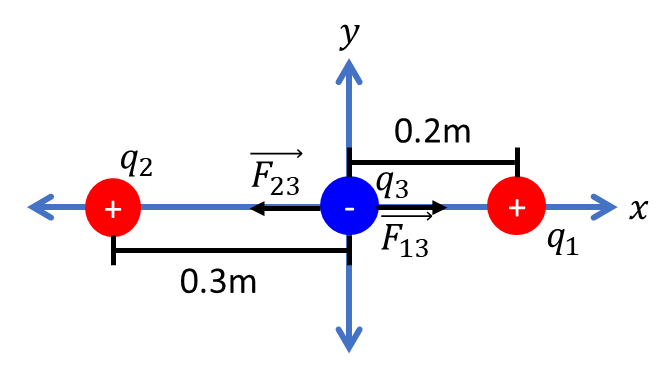
\includegraphics[width=.4\linewidth]{Imp4t1.png} 
			\end{center}
			$$ q_1 = 4nC = 4 \times 10^{-9}C, \quad q_2 = 5nC = 5 \times 10^{-9}C, \quad q_3 = -6nC = -6 \times 10^{-9}C $$
			$$ r_{13} = 0.2m, \quad r_{23} = 0.3m $$ \\
			$$ \vec{F_{t3}} = \vec{F_{13}} + \vec{F_{23}} $$
			$$ \vec{F_{13}} = k_e \frac{q_1q_3}{(r_{13})^2} \hat{r}, \quad \vec{F_{23}} = k_e \frac{q_2q_3}{(r_{23})^2} \hat{r} $$
			$$ \vec{F_{t3}} = k_e \frac{|q_1||q_3|}{(r_{13})^2} \hat{i} - \vec{F_{23}} = k_e \frac{|q_2||q_3|}{(r_{23})^2} \hat{i} $$ \\
			$$ \vec{F_{13}} = 8.99 \times 10^9 \frac{Nm^2}{C^2} \left(  \frac{(4 \times 10^{-9}C)(6 \times 10^{-9}C)}{(0.2m)^2} \right) \hat{i} $$
			$$ \vec{F_{13}} = 8.99 \times 10^9 \frac{Nm^2}{C^2} \left(  \frac{2.4 \times 10^{-17}C^2}{0.04m^2} \right) \hat{i} $$
			$$ \vec{F_{13}} = \left(  \frac{2.1576 \times 10^{-7}Nm^2}{0.04m^2} \right) \hat{i} $$
			$$ \vec{F_{13}} = 5.394 \times 10^{-6}N \hat{i} $$ \\
			$$ \vec{F_{23}} = -8.99 \times 10^9 \frac{Nm^2}{C^2} \left(  \frac{(5 \times 10^{-9}C)(6 \times 10^{-9}C)}{(0.3m)^2} \right) \hat{i} $$
			$$ \vec{F_{23}} = -8.99 \times 10^9 \frac{Nm^2}{C^2} \left(  \frac{3 \times 10^{-17}C^2}{0.09m^2} \right) \hat{i} $$
			$$ \vec{F_{23}} = -\left(  \frac{2.697 \times 10^{-7}Nm^2}{0.09m^2} \right) \hat{i} $$
			$$ \vec{F_{23}} = -2.99667 \times 10^{-6}N \hat{i} $$ \\
			$$ \vec{F_{t3}} = \vec{F_{13}} + \vec{F_{23}} $$
			$$ \vec{F_{t3}} = 5.394 \times 10^{-6}N \hat{i} - 2.99667 \times 10^{-6}N \hat{i} $$
			$$ \vec{F_{t3}} = 2.4 \times 10^{-6}N \hat{i} $$
			$$ \underline{F_{t3} = 2.4 \times 10^{-6}N \; a \; 0^0} $$

		\section{Problema 5:}\label{sec:Problema5}
			Considera dos cargas puntuales $ q_1 $ y $ q_2 $ con la misma magnitud pero con signos
			opuestos separados por una distancia $ d $. Ahora calcula la fuerza electrostática sobre
			una carga $ Q $ positiva localizada en un punto $ P $ sobre una linea perpendicular a la
			linea que separa a los dos cargas y que pase por el punto medio. Como segundo paso,
			supón que la posición de $ Q $ tiende hacia infinito. ¿Cuál es el límite de la expresión
			para la fuerza electrostática sobre $ Q $ en este caso?.	
			\begin{center}
				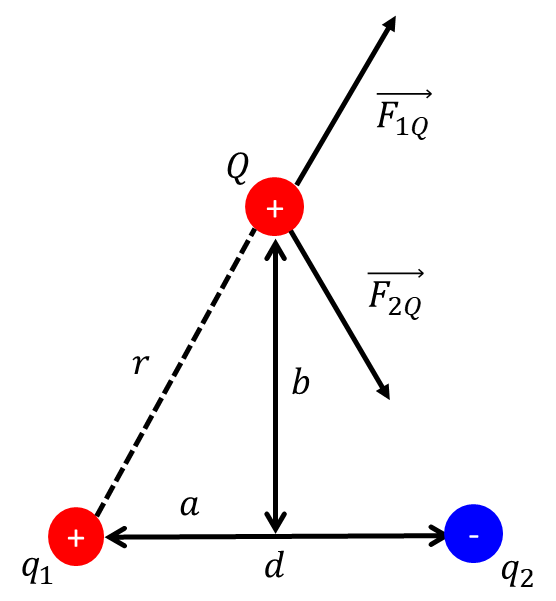
\includegraphics[width=.4\linewidth]{Imp5t1.png} 
			\end{center}
			$$ a = \frac{d}{2}, \quad |q_1| = |q_2| = |q| $$
			$$ r_{1Q} = \sqrt{a^2+b^2}, \quad r_{2Q} = \sqrt{a^2+b^2} $$ \\
			$$ \vec{F_{eQ}} = \vec{F_{1Q}} + \vec{F_{2Q}} $$
			$$ \vec{F_{1Q}} = \vec{F_{1Q}}x + \vec{F_{1Q}}y, \quad \vec{F_{2Q}} = \vec{F_{2Q}}x + \vec{F_{2Q}}y$$
			$$ \vec{F_{1Q}} = k_e \frac{|q_1||Q|}{(r_{1Q})^2} \hat{i} + k_e \frac{|q_1||Q|}{(r_{1Q})^2} \hat{j}, \quad 
			\vec{F_{2Q}} = k_e \frac{|q_2||Q|}{(r_{2Q})^2} \hat{i} - k_e \frac{|q_2||Q|}{(r_{2Q})^2} \hat{j}$$
			$$ \vec{F_{eQ}} = \left( k_e \frac{|q_1||Q|}{(r_{1Q})^2} \hat{i} + k_e \frac{|q_1||Q|}{(r_{1Q})^2} \hat{j} \right) 
			+ \left( k_e \frac{|q_2||Q|}{(r_{2Q})^2} \hat{i} - k_e \frac{|q_2||Q|}{(r_{2Q})^2} \hat{j} \right) $$ \\
			$$ \vec{F_{1Q}} = k_e \frac{|q_1||Q|}{(\sqrt{a^2+b^2})^2} \hat{i} + k_e \frac{|q_1||Q|}{(\sqrt{a^2+b^2})^2} \hat{j} $$
			$$ \vec{F_{1Q}} = k_e \frac{|q||Q|}{a^2+b^2} \hat{i} + k_e \frac{|q||Q|}{a^2+b^2} \hat{j} $$
			$$ \vec{F_{1Q}}x = k_e \frac{|q||Q|}{a^2+b^2} \hat{i}, \quad \vec{F_{1Q}}y = k_e \frac{|q||Q|}{a^2+b^2} \hat{j} $$ \\
			$$ \vec{F_{2Q}} = k_e \frac{|q_2||Q|}{(\sqrt{a^2+b^2})^2} \hat{i} - k_e \frac{|q_2||Q|}{(\sqrt{a^2+b^2})^2} \hat{j} $$
			$$ \vec{F_{2Q}} = k_e \frac{|q||Q|}{a^2+b^2} \hat{i} - k_e \frac{|q||Q|}{a^2+b^2} \hat{j} $$
			$$ \vec{F_{2Q}}x = k_e \frac{|q||Q|}{a^2+b^2} \hat{i},\quad \vec{F_{2Q}}y = -k_e \frac{|q||Q|}{a^2+b^2} \hat{j} $$ \\
			$$ \vec{F_{1Q}} = \vec{F_{1Q}}x + \vec{F_{1Q}}y, \quad \vec{F_{2Q}} = \vec{F_{2Q}}x + \vec{F_{2Q}}y$$
			$$ \vec{F_{eQ}} = \left( k_e \frac{|q||Q|}{a^2+b^2} \hat{i} + k_e \frac{|q||Q|}{a^2+b^2} \hat{j} \right) 
			+ \left( k_e \frac{|q||Q|}{a^2+b^2} \hat{i} - k_e \frac{|q||Q|}{a^2+b^2} \hat{j} \right) $$ 
			$$ \vec{F_{eQ}} = \left( k_e \frac{|q||Q|}{a^2+b^2} \hat{i} + k_e \frac{|q||Q|}{a^2+b^2} \hat{i} \right) 
			+ \left( k_e \frac{|q||Q|}{a^2+b^2} \hat{j} - k_e \frac{|q||Q|}{a^2+b^2} \hat{j} \right) $$
			$$ \vec{F_{eQ}} = \left( 2k_e \frac{|q||Q|}{a^2+b^2} \hat{i} \right) + (0 \hat{j}) $$
			$$ \vec{F_{eQ}} = \left( 2k_e \frac{|q||Q|}{(\frac{d}{2})^2+b^2} \hat{i} \right) = \left( 2k_e \frac{|q||Q|}{\frac{d^2}{4}+b^2} \hat{i} \right) =
			\left( 2k_e \frac{|q||Q|}{\frac{d^2+4b^2}{4}} \hat{i} \right)$$
			$$ \underline{\vec{F_{eQ}} = 8k_e \frac{|q||Q|}{d^2+4b^2} \hat{i}} $$ \\
			Si la posición de $ Q $ tendiera hacia infinito podríamos decir que $ b \gg d $ por lo que al aplicar 
			esto a la ecuación obtenida tenemos que:
			$$ \vec{F_{eQ}} = 8k_e \frac{|q||Q|}{d^2+4b^2} \hat{i} = 8k_e \frac{|q||Q|}{4b^2} \hat{i} = \underline{2k_e \frac{|q||Q|}{b^2} \hat{i}} $$ \\


		\section{Problema 6:}\label{sec:Problema6}
			A lo largo del eje $ x $ existe una línea de carga continua que se extiende desde $ x = x_0 $
			hasta infinito positivo. La línea tiene una densidad de carga lineal uniforme $ \lambda_0 $.
			¿Cuál es la magnitud y la dirección del campo eléctrico en el origen?.
			\begin{center}
				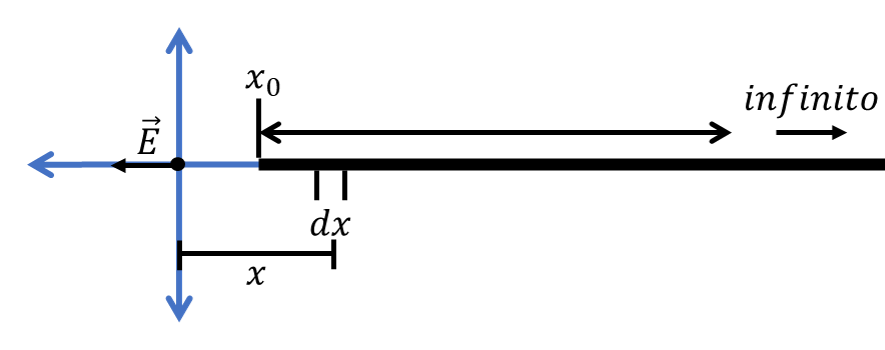
\includegraphics[width=.5\linewidth]{Imp6t1.png} 
			\end{center}
			$$ \lambda_0 = \frac{Q}{L}, \quad dq = \lambda_0 dx $$ \\
			$$ \vec{E} = k_e \int \frac{dq}{r^2} \hat{r} $$
			$$ \vec{E} = k_e \int_{x_0}^{\infty} \frac{\lambda_0 dx}{x^2} $$
			$$ \vec{E} = k_e \lambda_0 \int_{x_0}^{\infty} x^{-2}dx $$
			$$ \vec{E} = k_e \lambda_0 \left[ - \frac{1}{x} \right]_{x_0}^{\infty}$$
			$$ \vec{E} = k_e \lambda_0 \left[ - \frac{1}{\infty} - \left( -\frac{1}{x_0} \right) \right] $$
			$$ \vec{E} = k_e \lambda_0 \left[ (0) + \frac{1}{x_0} \right] $$
			$$ \vec{E} = -\frac{k_e \lambda_0}{x_0} \hat{i} $$
			$$ \vec{E} = \left( -\frac{k_e}{x_0} \right) \left( \frac{Q}{L} \right) $$ 
			$$ \vec{E} = -\frac{k_e Q}{x_0L} \hat{i} $$
			$$ \underline{E = \frac{k_e Q}{x_0L} \: a \: 180^0} $$\\
			
		\section{Problema 7:}\label{sec:Problema7}
			Una carga puntual de $ +2nC $ está en el origen y una segunda carga puntual de $ -5nC $
			está en el eje $ x $ en $ x = 0.8m $.
			\begin{center}
				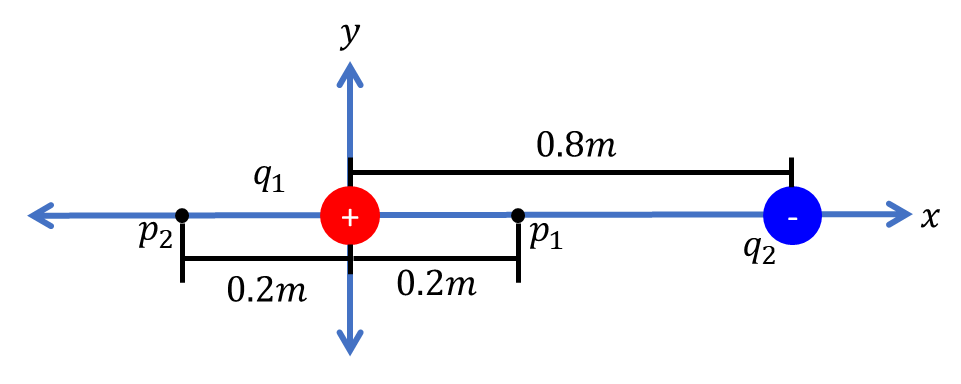
\includegraphics[width=.5\linewidth]{Imp7t1.png} 
			\end{center}
			$$ q_1 = 2nc = 2 \times 10^{-9}C, \quad q_2 = -5nC = -5 \times 10{-9}C $$
			$$ r_{1p_1} = 0.2m, \quad r_{1p_2} = 0.2m $$
			$$ r_{2p_1} = 0.8m - 0.2m = 0.6m , \quad r_{2p_2} = 0.8m + 0.2m = 1m $$
				\begin{enumerate}
					\item[a)]	Encuentra el campo eléctrico (vector, magnitud y dirección) en los
							puntos $ x = 0.2m $ y $ x = -0.2m $. 
							$$ \vec{E} = k_e \frac{|q|}{r^2} \hat{r} $$ \\
							\textbf{Carga 1, Punto 1:}
							$$ \vec{E_{1p_1}} = k_e \frac{|q_1|}{(r_{1p_1})^2} \hat{i} $$
							$$ \vec{E_{1p_1}} = 8.99 \times 10^9 \frac{Nm^2}{C^2} \left( \frac{2 \times 10^{-9}C}{(0.2m)^2} \right) \hat{i} $$
							$$ \vec{E_{1p_1}} = \left( \frac{17.98 \frac{Nm^2}{C}}{0.04m^2} \right) \hat{i} $$
							$$ \vec{E_{1p_1}} = 449.5 \frac{N}{C} \hat{i} $$ \\
							\textbf{Carga 2, Punto 1:}
							$$ \vec{E_{2p_1}} = -k_e \frac{|q_2|}{(r_{2p_1})^2} \hat{i} $$
							$$ \vec{E_{2p_1}} = -8.99 \times 10^9 \frac{Nm^2}{C^2} \left( \frac{5 \times 10{-9}C}{(0.6m)^2} \right) \hat{i} $$
							$$ \vec{E_{2p_1}} = -\left( \frac{44.95 \frac{Nm^2}{C}}{0.36m^2} \right) \hat{i} $$
							$$ \vec{E_{2p_1}} = -124.861 \frac{N}{C} \hat{i} $$ \\
							\textbf{Campo eléctrico total en punto 1:}
							$$ \vec{E_{tp_1}} = \vec{E_{1p_1}} + \vec{E_{2p_1}} $$
							$$ \vec{E_{tp_1}} = 449.5 \frac{N}{C} \hat{i} - 124.861 \frac{N}{C} \hat{i} $$
							$$ \underline{\vec{E_{tp_1}} = 324.639 \frac{N}{C} \hat{i}} $$
							$$ \underline{E_{tp_1} = 324.639 \frac{N}{C} \; a \; 0^0} $$ \\
							\textbf{Carga 1, Punto 2:}
							$$ \vec{E_{1p_2}} = -k_e \frac{|q_1|}{(r_{1p_2})^2} \hat{i} $$
							$$ \vec{E_{1p_2}} = -8.99 \times 10^9 \frac{Nm^2}{C^2} \left( \frac{2 \times 10^{-9}C}{(0.2m)^2} \right) \hat{i} $$
							$$ \vec{E_{1p_2}} = -\left( \frac{17.98 \frac{Nm^2}{C}}{0.04m^2} \right) \hat{i} $$
							$$ \vec{E_{1p_2}} = -449.5 \frac{N}{C} \hat{i} $$ \\
							\textbf{Carga 2, Punto 2:}
							$$ \vec{E_{2p_2}} = -k_e \frac{|q_2|}{(r_{2p_2})^2} \hat{i} $$
							$$ \vec{E_{2p_2}} = -8.99 \times 10^9 \frac{Nm^2}{C^2} \left( \frac{5 \times 10{-9}C}{(1m)^2} \right) \hat{i} $$
							$$ \vec{E_{2p_2}} = -\left( \frac{17.98 \frac{Nm^2}{C}}{1m^2} \right) \hat{i} $$
							$$ \vec{E_{2p_2}} = -17.98 \frac{N}{C} \hat{i} $$ \\
							\textbf{Campo eléctrico total en punto 2:}
							$$ \vec{E_{tp_2}} = \vec{E_1{p_2}} + \vec{E_{2p_2}} $$
							$$ \vec{E_{tp_2}} = -449.5 \frac{N}{C} \hat{i} - 17.98 \frac{N}{C} \hat{i}$$
							$$ \underline{\vec{E_{tp_2}} = -467.48 \frac{N}{C} \hat{i}} $$
							$$ \underline{E_{tp_2} = 467.48 \frac{N}{C} \; a \; 180^0} $$ \\


					\item[b)]	Calcula la fuerza eléctrica neta que las dos cargas ejercerían sobre
							un electrón (carga negativa) colocado en cada punto del enciso a). \\
							Carga de un electrón = $ -1.6021765 \times 10^{-19}C $
							$$ \vec{F_e} = q_0 \vec{E} $$ \\
							\textbf{Fuerza eléctrico neta en punto 1:}
							$$ \vec{F_{np_1}} = q_e \vec{E_{tp_1}} $$
							$$ \vec{F_{np_1}} = (-1.6021765 \times 10^{-19}C) (324.639 \frac{N}{C} \hat{i}) $$
							$$ \underline{\vec{F_{np_1}} = -5.20 \times 10^{-17}N \hat{i}} $$
							\textbf{Fuerza eléctrico neta en punto :}
							$$ \vec{F_{np_1}} = q_e \vec{E_{tp_2}} $$
							$$ \vec{F_{np_1}} = (-1.6021765 \times 10^{-19}C) (-467.48 \frac{N}{C} \hat{i}) $$
							$$ \underline{\vec{F_{np_1}} = 7.49 \times 10^{-17}N \hat{i}} $$
				\end{enumerate}

		\section{Problema 8:}\label{sec:Problema8}
			Dos partículas con cargas $ q_1 = 0.5nC $ y $ q_2 = 8nC $ están separadas por una distancia
			de $ 1.2m $ ¿En qué punt de la línea que conecta las dos cargas, el campo eléctrico
			total producido por ambas cargas es igual a cero?.
			está en el eje $ x $ en $ x = 0.8m $.
			\begin{center}
				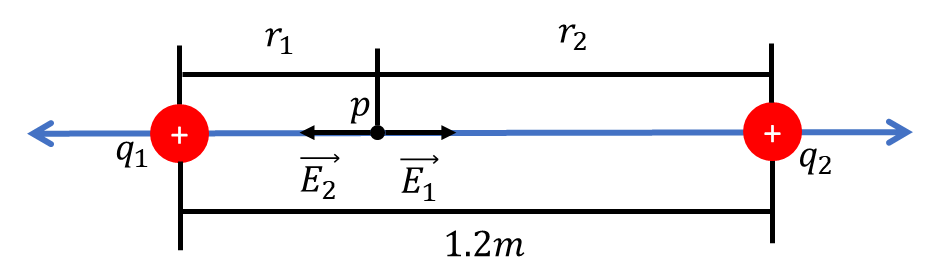
\includegraphics[width=.5\linewidth]{Imp8t1.png} 
			\end{center}
			$$ q_1 = 0.5nc = 0.5 \times 10^{-9}C, \quad q_2 = 8nC = 8 \times 10{-9}C $$
			$$ r_1 = 1.2m - r_2, \quad r_2 = 1.2m - r_1 $$
			$$ \vec{E} = k_e \frac{|q|}{r^2} \hat{r} $$
			$$ \vec{E_1} = \vec{E_2} $$
			$$ k_e \frac{|q_1|}{(r_1)^2} = k_e \frac{|q_2|}{(r_2)^2} $$
			$$ 8.99 \times 10^9 \frac{Nm^2}{C^2} \left( \frac{0.5 \times 10^{-9}C}{(r_1)^2} \right) = 
			8.99 \times 10^9 \frac{Nm^2}{C^2} \left( \frac{8 \times 10{-9}C}{(1.2m - r_1)^2} \right) $$
			$$ \frac{4.495 \frac{Nm^2}{C}}{(r_1)^2} = \frac{71.92 \frac{Nm^2}{C}}{(1.2m - r_1)^2} $$
			$$ 4.495 \frac{Nm^2}{C}(1.2m - (r_1)^2) = 71.92 \frac{Nm^2}{C}((r_1)^2) $$
			$$ 5.394 \frac{Nm^3}{C} - 4.495(r_1)^2 \frac{Nm^2}{C} = 71.92(r_1)^2 \frac{Nm^2}{} $$
			$$ -71.92(r_1)^2 \frac{Nm^2}{C} - 4.495(r_1)^2 \frac{Nm^2}{C} = -5.394 \frac{Nm^3}{C} $$
			$$ -76.415(r_1)^2 \frac{Nm^2}{C}  = -5.394 \frac{Nm^3}{C} $$
			$$ (r_1)^2 = \frac{-5.394 \frac{Nm^3}{C}}{-76.415\frac{Nm^2}{C}} $$
			$$ r_1 = \sqrt{7.06 \times 10^{-2}}m $$
			$$ \underline{r_1 = .266 m}, \quad r_1 ? -.266 m $$ \\

		\section{Problema 9:}\label{sec:Problema9}
			Se proyecta un electrón a una velocidad de $ v_0 = 5.83 \times 10^6 m/s $ a un ángulo de $ 39^0 $.
			Se tiene $ E = 1870N/C $ dirigido hacia arriba, $ d = 1.97cm $ y $ L = 6.20cm $. ¿El electrón
			golpeará una de las placas?, si lo hace, ¿cuál de ellas golpeará y a qué distancia
			del lado izquierdo?.
			\begin{center}
				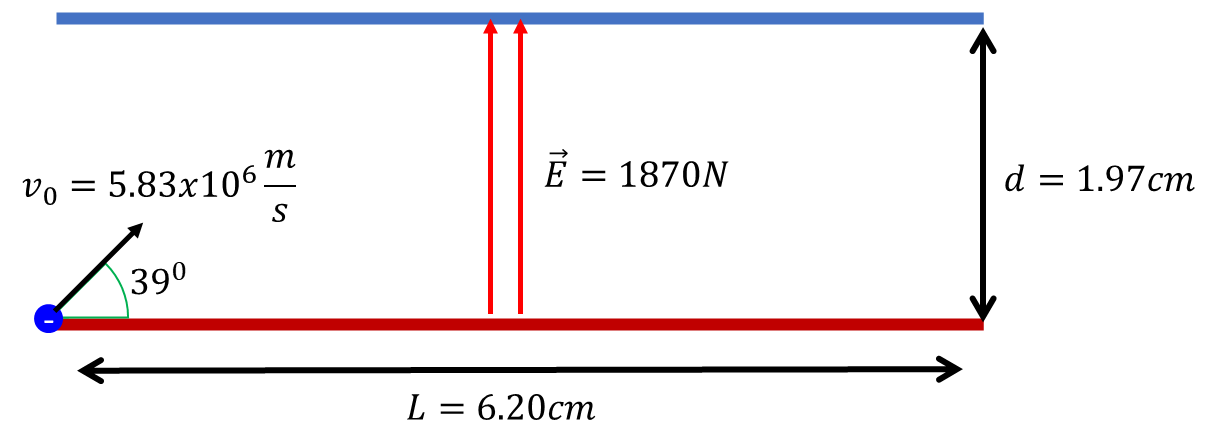
\includegraphics[width=.6\linewidth]{Imp9t1.png} 
			\end{center}
			Carga de un electrón = $ -1.6021765 \times 10^{-19}C $\\
			Masa de un electrón = $ 9.1094 \times 10^{-31} kg $
			$$ d = 1.97cm = 0.0197m, \quad L = 6.20cm = 0.062m $$ \\
			$$ v_0 = 5.83 \times 10^6m/s $$
			$$ v_0x = 5.83 \times 10^6m/s \cos(39) = 4.53 \times 10^6m/s \hat{i} $$
			$$ v_0y = 5.83 \times 10^6m/s \sin(39) = 3.67 \times 10^6m/s \hat{i} $$ \\
			$$ \vec{F_e} = q_e \vec{E} = m \vec{a} $$
			$$ (-1.6021765 \times 10^{-19}C)(1870N/C \hat{j}) = (9.1094 \times 10^{-31}kg) \vec{a}$$
			$$ -2.99607 \times 10^{-16}N \hat{j} = (9.1094 \times 10^{-31}kg) \vec{a} $$
			$$ \vec{a} = \frac{-2.99607 \times 10^{-16}N \hat{j}}{9.1094 \times 10^{-31}kg} $$
			$$ \vec{a} = -3.289 \times 10^{14} m/s^2 \hat{j} $$ \\

			$$ d = v_0yt -1/2at^2 $$
			$$ 0.0197m = 3.67 \times 10^6t - 1/2(3.289 \times 10^{14} m/s^2)t^2 $$
			$$ 1.6445 \times 10^{14} - 3.67 \times 10^6t + 0.0197 = 0  $$
			$$ \frac{-b \pm \sqrt{b^2-4ac}}{2a} $$
			$$ \frac{3.67 \times 10^6 \pm \sqrt{(- 3.67 \times 10^6)^2 - 4(1.6445 \times 10^{14})(0.0197)}}{2(1.6445 \times 10^{14})} $$
			$$ \frac{3.67 \times 10^6 \pm \sqrt{5.102 \times 10^{11}}}{3.289 \times 10^{14}} $$
			$$ t_1 = \frac{3.67 \times 10^6 + \sqrt{5.102 \times 10^{11}}}{3.289 \times 10^{14}} , \quad 
			t_2 = \frac{3.67 \times 10^6 - \sqrt{5.102 \times 10^{11}}}{3.289 \times 10^{14}} $$
			$$ t_1 = 1.33301 \times 10^{-8}s, \quad t_2 = 8.98667 \times 10^{-9}s $$ \\
			$$ x = v_0xt $$
			$$ x = (4.53 \times 10^{6}m/s)(8.98667 \times 10^{-9}s) $$
			$$ x = 0407m $$
			Por lo tanto no toca ningún plano ya que cuando el electrón llega a la altura de d en x ya no esta dentro de los planos

		\section{Problema 10:}\label{sec:Problema10}
			Tres cilindros sólidos de plástico tienen un radio de $ 2.50cm $ y una longitud de
			$ 6.00cm $.  Determine la carga de cada uno.
				\begin{enumerate}
					\item[a)]	Uno está cargado con una densidad uniforme $ 15.0 nC/m^2 $ en toda su
					superficie.
					\item[b)]	Otro está cargado con la misma densidad uniforme sólo en su superficie
					lateral curva.
					\item[c)] El tercero está cargado con una densidad uniforme de $ 500 nC/m^3 $
					en todo el plástico.
				\end{enumerate}
     
	\end{document}